\documentclass[12pt, a4paper, oneside]{ctexart}
\usepackage{amsmath, amsthm, amssymb, bm, graphicx, hyperref, mathrsfs}

\title{\textbf{结构化学\ 综合作业1}}
\author{刘之翔 \ \ 朱德航 \ \ 何文龙}
\date{\today}
\linespread{1.25}
\newcounter{problemname}
\newenvironment{problem}{\stepcounter{problemname}\par\noindent\textbf{题目\arabic{problemname}. }}{\\\par}
\newenvironment{solution}{\par\noindent\textbf{解答. }}{\\\par}
\newenvironment{note}{\par\noindent\textbf{题目\arabic{problemname}的注记. }}{\\\par}

\begin{document}

\maketitle

\begin{problem}
    2维平面上运动的粒子,受到如图所示的势能限制.
    \begin{equation}
        V = 
    \begin{cases}
        0,\quad -\frac b2< x < \frac b 2 \text{and} -\frac a 2  < y < \frac a 2\\
        \infty , x \ge \frac b 2\  \text{or} \ x \le - \frac b 2 \ \text{or} \ -\frac b 2 < x < \frac{b} 2\ \text{and}\ y \ge \frac a 2\ \text{or}\ y \le -\frac a 2
        \end{cases}
    \end{equation}

    求:

    \begin{enumerate}
        \item 箱中的波函数 $\psi$ 表达式
        \item 能级E表达式
        \item 绘制前6个轨道的波函数图形
        \item 计算粒子在箱中的平均位置和平均动量
    \end{enumerate}
\end{problem}


\begin{solution}

    \paragraph{1.1}

    对于箱中势能
    \begin{equation}
        V(x,y)=0
    \end{equation}

    列出薛定谔方程
    \begin{equation}
        -\frac{h^2}{8\pi^2 m}\left ( \frac{\partial^2}{\partial x^2} +\frac{\partial^2}{\partial y^2}\right ) \psi=E\psi
    \end{equation}

    对$\psi$进行变量分离
    \begin{equation}
        \psi=\psi(x,y)=X(x)Y(y)
    \end{equation}

    代入方程
    \begin{equation}
        -\frac{h^2}{8\pi^2 m}\left ( \frac{\partial^2}{\partial x^2} +\frac{\partial^2}{\partial y^2}\right ) XY=EXY
    \end{equation}

    整理得
    \begin{equation}
        -\frac{h^2}{8\pi^2 m}\frac{\partial^2X}{X\partial x^2}=E+\frac{h^2}{8\pi^2 m}  \frac{\partial^2Y}{Y\partial y^2}
    \end{equation}

    定义x分量的能量为Ex,y分量的能量为Ey
    \begin{equation}
        E_x = -\frac{h^2}{8\pi^2 m}\frac{\partial^2X}{X\partial x^2}=E+\frac{h^2}{8\pi^2 m} \frac{\partial^2Y}{Y\partial y^2}
    \end{equation}
    \begin{equation}
        E_y = -\frac{h^2}{8\pi^2 m}\frac{\partial^2Y}{Y\partial y^2}=E+\frac{h^2}{8\pi^2 m} \frac{\partial^2X}{X\partial x^2}
    \end{equation}

    即可得
    \begin{equation}
        E=E_x+E_y
    \end{equation}

    分别求解本征函数
    \begin{equation}
        X(x)=\sqrt{\frac2b}\sin\frac{n_x\pi (x+b/2)}{b}\quad E_x=\frac{n_x^2h^2}{8mb^2}
    \end{equation}
    \begin{equation}
        Y(y)=\sqrt{\frac2a}\sin\frac{n_y\pi (y+a/2)}{a}\quad E_y=\frac{n_y^2h^2}{8ma^2}
    \end{equation}

    可得
    \begin{equation}
        \psi=X(x)Y(y)=\sqrt{\frac{4}{ab}}\sin\frac{n_x\pi (x+b/2)}{b}\sin\frac{n_y\pi (y+a/2)}{a}
    \end{equation}

    \paragraph{1.2}

    根据方程9、10、11可得
    \begin{equation}
        E=E_x+E_y=\frac{h^2}{8m}(\frac{n_x^2}{a^2}+\frac{n_y^2}{b^2})
    \end{equation}

    \paragraph{1.3}
    
    前6个波函数轨道图,使用python matplotlib 绘制,代码见附录。

    为了方便,在代码中令a=b=3代入运算

    \begin{figure}[h]
        \centering
        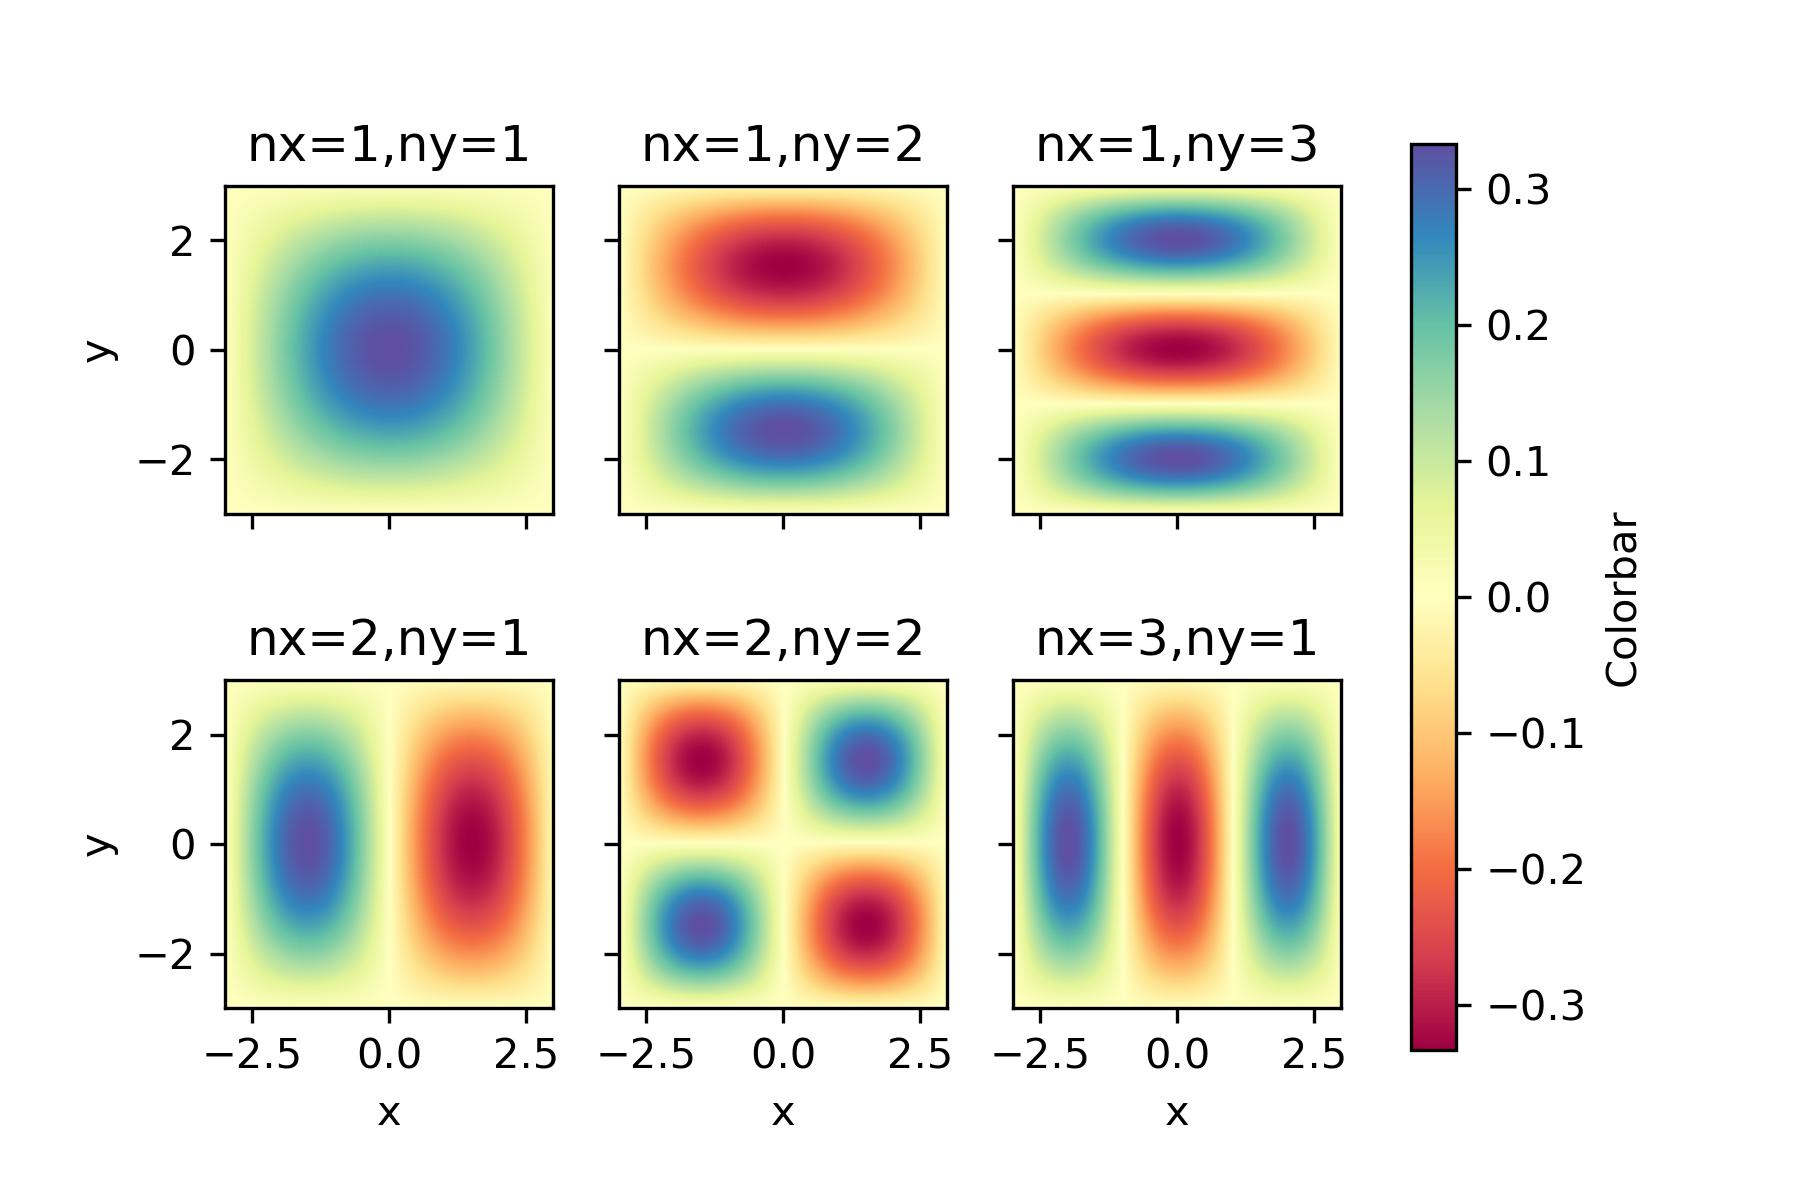
\includegraphics{WaveFunction.jpg}
        \caption{二维势箱运动粒子前6个轨道的波函数图形}
    \end{figure}

\

\

\

\

\

    \paragraph{1.4}
    根据算符定义可得坐标平均值的表达式
    \begin{equation}
        \langle x \rangle = \int _{-b/2}^{b/2}\psi^*x\psi dx 
    \end{equation}

    代入波函数可得
    \begin{align}
        \langle x \rangle &= \int _{-b/2}^{b/2} \sqrt{\frac{4}{ab}}\sin\frac{n_x\pi (x+b/2)}{b}\sin\frac{n_y\pi (y+a/2)}{a} x \sqrt{\frac{4}{ab}}\sin\frac{n_x\pi (x+b/2)}{b}\sin\frac{n_y\pi (y+a/2)}{a} dx \\
        &= \frac{4}{ab}\sin^2\frac{n_y\pi (y+a/2)}{a} \int _{-b/2}^{b/2} x \sin^2\frac{n_x\pi (x+b/2)}{b} dx\\
    \end{align}

    代换z=x+b/2
    \begin{align}
        \langle x \rangle &= \frac{4}{ab}\sin^2\frac{n_y\pi (y+a/2)}{a} \int_0^b \sin^2\frac{n_x\pi z}{b}(z-\frac b 2) dz\\
        &= \frac{4}{ab}\sin^2\frac{n_y\pi (y+a/2)}{a} \left ( \int_0^b z\sin^2\frac{n_x\pi z}{b} dz- \frac b 2 \int_0^b z\sin^2\frac{n_x\pi z}{b} dz \right )\\
        &=  \frac{4}{ab}\sin^2\frac{n_y\pi (y+a/2)}{a} \left (\frac {b^2}{4}- \frac {b^2}{4}  \right )\\
        &= 0 \\
    \end{align}

    同理可得
    \begin{equation}
        \langle y \rangle = 0
    \end{equation}

    根据动量算符定义
    \begin{equation}
        \langle P_x \rangle = \frac{ih}{2\pi} \frac{d}{dx}
    \end{equation}
    
    代入波函数可得
    \begin{align}
        \langle P_x \rangle &= \frac{4}{ab}\sin^2\frac{n_y \pi (y+a/2)}{a} \int _{-b/2}^{b/2} \sin \frac{n_x \pi(x+b/2)}{b} \frac{ih}{2\pi} \frac{d}{dx} \sin \frac{n_x \pi(x+b/2)}{b} dx \\
        &=  \frac{4}{ab}\sin^2\frac{n_y \pi (y+a/2)}{a} \int _{-b/2}^{b/2} \sin \frac{n_x \pi(x+b/2)}{b} \frac{ih}{2\pi} d \sin \frac{n_x \pi(x+b/2)}{b}\\
        &= 0 \\
    \end{align}

    同理可得
    \begin{equation}
        \langle P_y \rangle = 0
    \end{equation}

\end{solution}

\begin{problem}
    根据一维箱中粒子模型及其解的结论,将其推广至有限深度势箱,只考虑束缚态。
    \begin{enumerate}
        \item 讨论势箱宽度与波函数的形式以及相邻本征值的差值之间的关系。
        \item 讨论势箱深度与波函数的形式以及相邻本征值的差值志坚的关系。
    \end{enumerate}
    
\end{problem}

\begin{solution}
    \paragraph{}
        对于有限深势阱
    \begin{equation}
        V(x) = 
        \begin{cases}
            V_0,\quad x < -\frac a 2 \\
            0 , \quad -\frac a2 \le x \ge \frac a 2\\
            V_0, \quad x > \frac a 2
            \end{cases}
    \end{equation}

        考虑束缚态 $ 0<E<V_0$

        对于I、III区域
        \begin{equation}
            \hat H_I=\hat H_{\text{III}}=(-\frac{\hbar^2}{2m}\nabla^2+V_0)
        \end{equation}       
        
        可得定态薛定谔方程
        \begin{equation}
            -\frac{\hbar^2}{2m}\frac{d^2}{dx^2}\psi+V_0\psi=E\psi 
        \end{equation}
        \begin{equation}
            \frac{d^2 \psi}{dx^2}-\frac{2m}{\hbar^2}(V_0-E)\psi=0
        \end{equation}

        令$\frac{2m}{\hbar^2}(V_0-E)=\beta^2$可得
        \begin{equation}
            \frac{d^2 \psi}{dx^2}-\beta^2\psi=0
        \end{equation}

        解得
        \begin{equation}
            \psi(x)=Ae^{\beta x}+Be^{-beta x}
        \end{equation}

        根据波函数的品优要求$\psi(x)|_{x \to \pm \infty}$ue qu
        \begin{equation}
            \psi(x) = 
            \begin{cases}
                Ae^{\beta x},\quad x < -\frac a 2 \\
                Be^{-\beta x} ,\quad x > \frac a 2
                \end{cases}
        \end{equation}

        对于II区域,同理可得定态薛定谔方程
        \begin{equation}
            \frac{d^2 \psi}{dx^2}+\frac{2m}{\hbar^2}E\psi=0
        \end{equation}

        令$\frac{2m}{\hbar^2}E = k^2$可得
        \begin{equation}
            \frac{d^2 \psi}{dx^2}+k^2\psi=0
        \end{equation}

        解得
        \begin{equation}
            \psi(x)=C\sin{k x}+D\cos{k x}
        \end{equation}

        又根据波函数的品优要求,连续可微,根据方程(36)得到I、III区域的解,可得到在区域交接处的边界条件
        \begin{equation}
            \psi(x)(a/2+0)=\psi(a/2-0)
        \end{equation}
        \begin{equation}
            \psi(x)(-a/2+0)=\psi(-a/2-0)
        \end{equation}
        \begin{equation}
            \frac{d\psi}{dx}(a/2+0)=\frac{d\psi}{dx}(a/2-0)
        \end{equation}
        \begin{equation}
            \frac{d\psi}{dx}(-a/2+0)=\frac{d\psi}{dx}(-a/2-0)
        \end{equation}

        综上条件可得,对于波函数有奇宇称偶宇称两种情况

        对于偶宇称
            \begin{equation}
                \psi(x)=C\cos kx
            \end{equation}
            
        根据边界条件解得
            \begin{equation}
                k\tan \frac{ka}2 = \beta
            \end{equation}

        令$ \epsilon = \frac{ka}2, \ \eta = \frac{\beta a}2 $
            \begin{equation}
                \epsilon \tan \epsilon = \eta
            \end{equation}
        
        代入$\epsilon$ 和$\eta $的定义,令等式右边常数等于$\epsilon_0$
            \begin{equation}
                \epsilon^2+\eta^2 = \frac{mV_0a^2}{2\hbar^2} = \epsilon_0^2
            \end{equation}

        可得
            \begin{equation}
                \epsilon \tan \epsilon = \sqrt{\epsilon_0^2-\epsilon^2}
            \end{equation}  
        方程的解,表示为两个函数的交点,作图求解
            \begin{equation}
                \tan \epsilon = \sqrt{\frac{\epsilon_0^2}{\epsilon^2}-1}
            \end{equation}

            \begin{figure}[h]
                \centering
                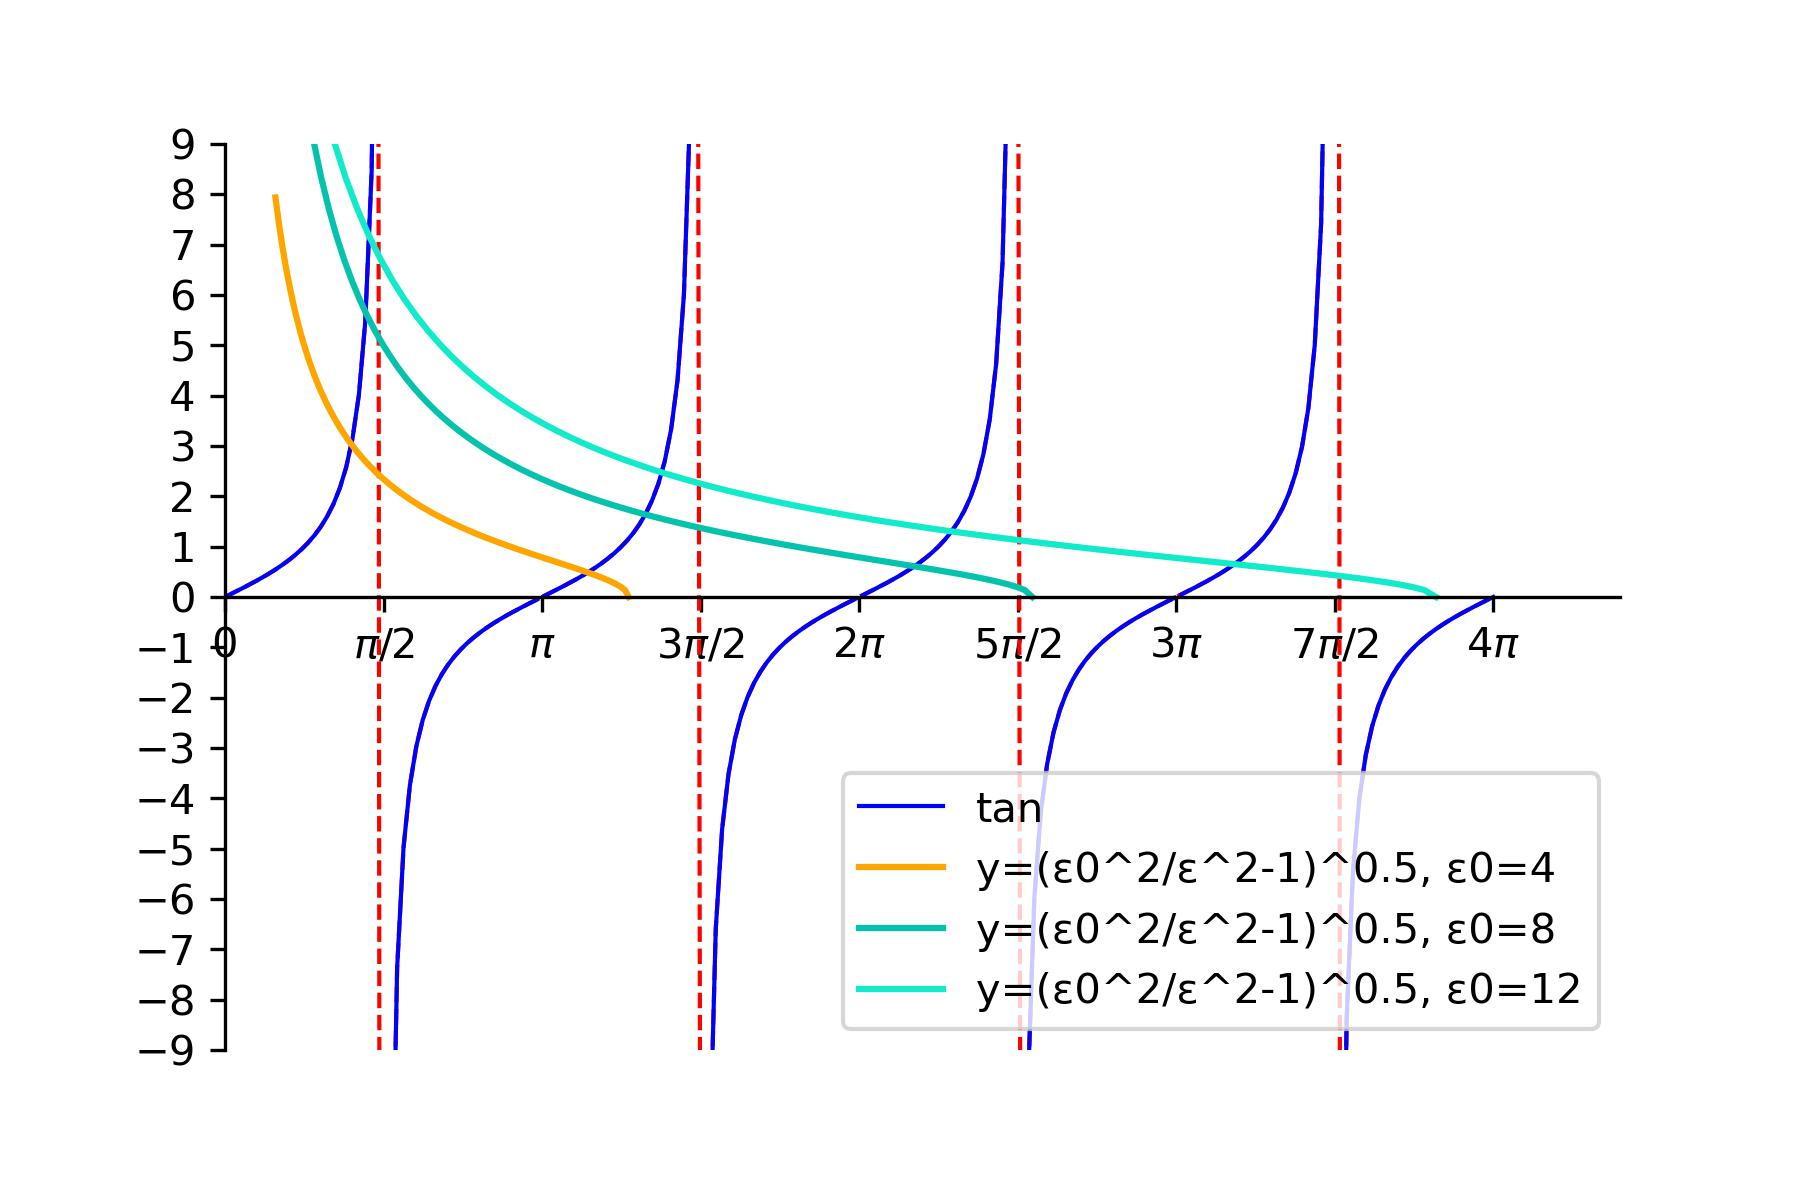
\includegraphics{Solution1.jpg}
                \caption{一维有限深势阱偶宇称波函数的作图求解}
            \end{figure}

        结合方程(47)可知,势箱宽度a与深度V0通过改变$\epsilon0$的取值来影响波函数本征值的个数与分布。a的平方与$\epsilon0$成正比,V0与$\epsilon0$成正比。而随着$\epsilon0$的增大,$ \sqrt{\frac{\epsilon_0^2}{\epsilon^2}-1}$ 与 $ \tan \epsilon$ 的交点变多,同时相邻本征值的差值也逐渐趋近于$\pi$。
        
        考虑极限情况,当V0足够深,a足够宽,则各本征值的差值等于$\pi$,而第一个本征值等于$\pi$,则可用n$\pi$(n为正整数)来表示所有本征值。此时该势阱演化为无限深势阱。
        
        对于奇宇称
        \begin{equation}
            \psi(x)=D\sin kx
        \end{equation}

        与偶宇称同理
        \begin{equation}
            -k \cot \frac{ka}2=\beta
        \end{equation}
        \begin{equation}
            \cot \epsilon = - \sqrt{\frac{\epsilon_0^2}{\epsilon^2}-1}
        \end{equation}


        同样作图求解
        \begin{figure}[h]
            \centering
            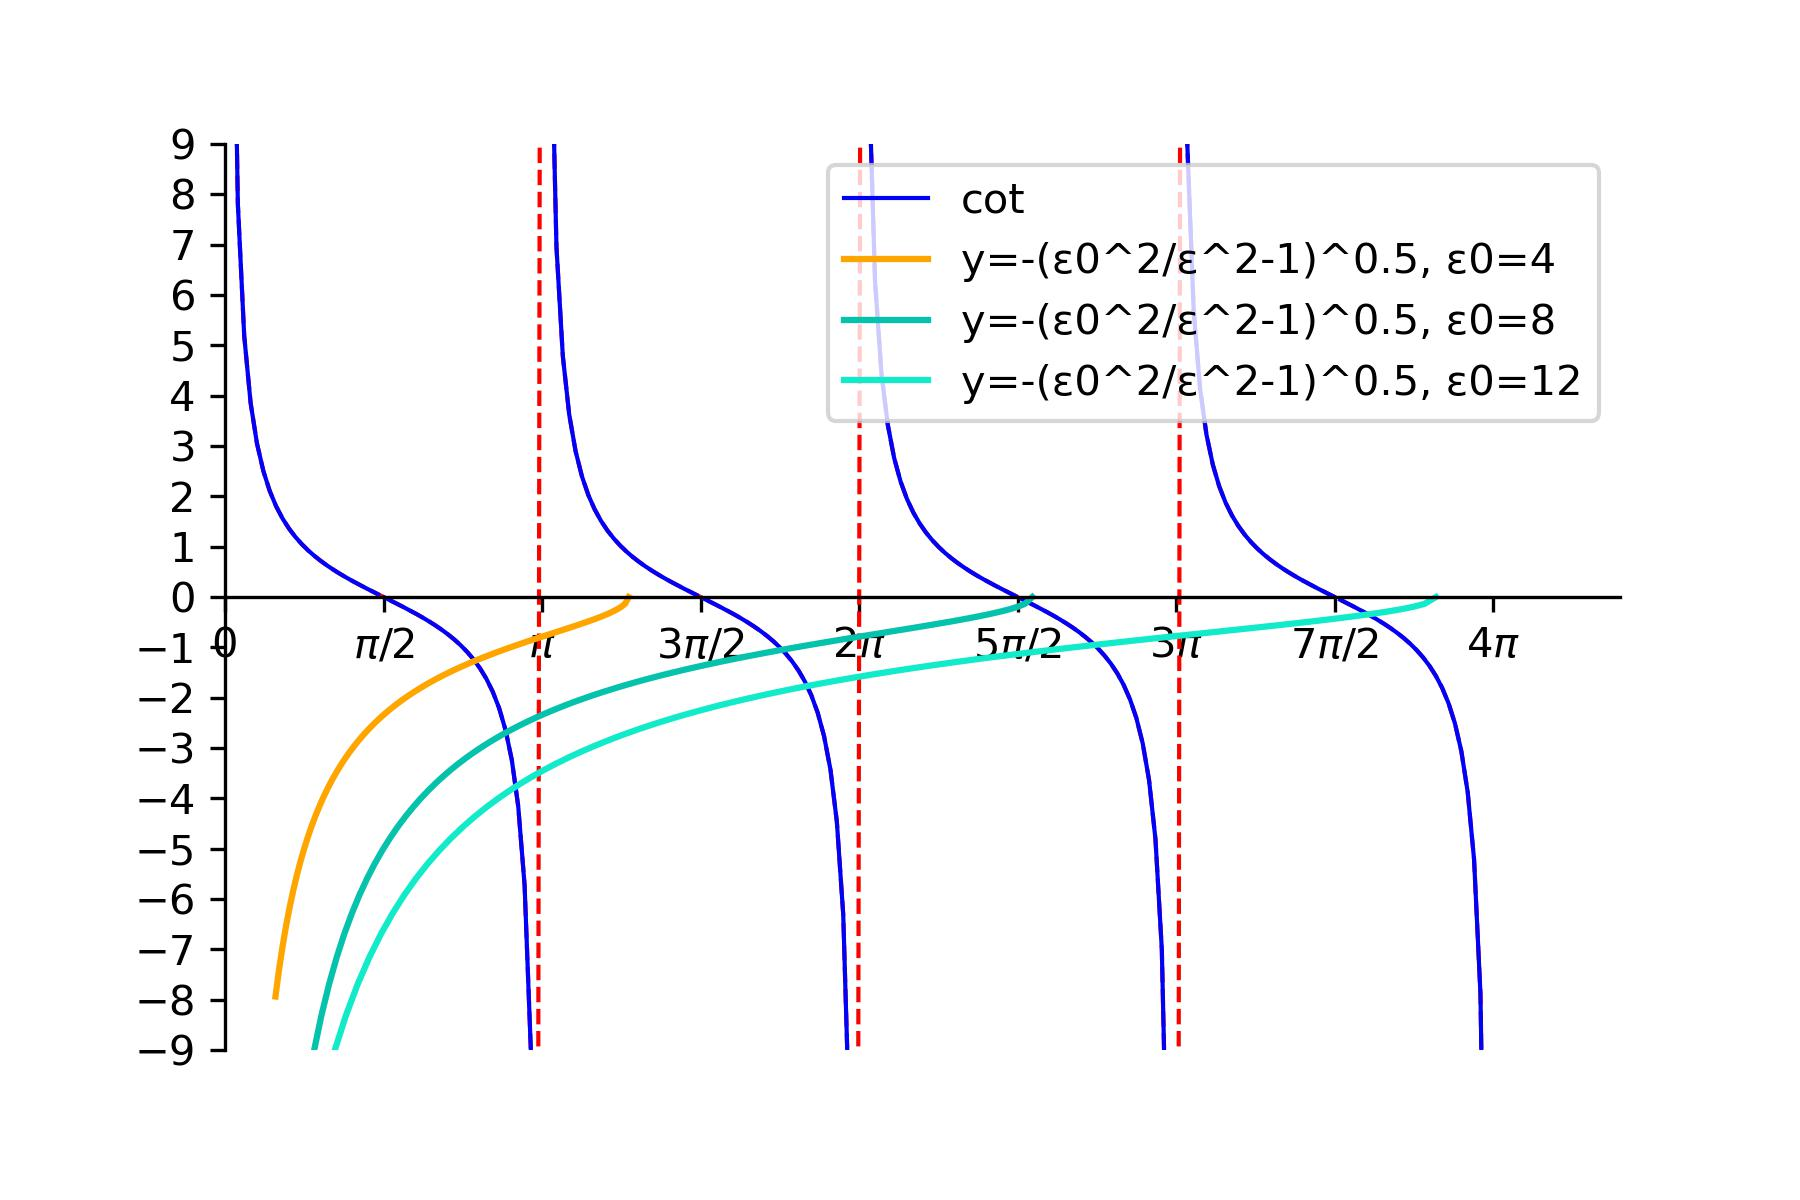
\includegraphics{Solution2.jpg}
            \caption{一维有限深势阱奇宇称波函数的作图求解}
        \end{figure}

        其性质与偶宇称类似。

\

\

\
\end{solution}

\begin{problem}
    结合讲义关于Plank公式和黑体辐射问题的回顾,吴有训先生事迹及网络资料,阅读Nobel奖获得者屠呦呦获奖感言和事迹及网络资料,撰写80-100字体会,与收集的资料一同上交。
\end{problem}

\begin{solution}
    在物理近代路上,无数伟人,Plank,吴有训,屠呦呦先生,巅峰而立,让我们知晓未来之路一何行:两袖清风文韬武略,一身正气教书育人,十年如一,或伏案籍之间,或奔走田之野,或守实验的夜,大胆假设,小心求证。科研无尽头,吾辈当勉行。
\end{solution}

% \begin{note}
%     这里是注记. 
% \end{note}

\newpage

\begin{thebibliography}{99}

    \bibitem{ref1}https://baike.baidu.com/item/\%E9\%A9\%AC\%E5\%85\%8B\%E6\%96\%AF\%C2\%B7\%E6\%99\%AE\%E6\%9C\%97 \\ \%E5\%85\%8B/990975
    \bibitem{ref2}http://www.gov.cn/zhuanti/2015-12/18/content\_5025361. htm
    \bibitem{ref3}https://www.nobelprize.org/prizes/medicine/2015/tu/prize-presentation/
    \bibitem{ref4}王友年,宋远红,张钰如。数学物理方法[M].大连理工大学出版社,2015
\end{thebibliography}

\newpage




\begin{appendices}
    \renewcommand{\thesection}{\Alph{section}}
    \section{附录}
    \paragraph{二维势箱波函数图形绘制代码}
    
    \begin{lstlisting}
        
    \end{lstlisting}
\end{appendices}

\end{document}

% \begin{equation}
        
% \end{equation}